\typeout{}\typeout{If latex fails to find aiaa-tc, read the README file!}

\documentclass[]{aiaa-tc}% insert '[draft]' option to show overfull boxes

\usepackage{mathptmx}         %CHANGE FONT TO TIMES NEW ROMAN
\usepackage{amsmath}          % for formula writing (i.e. 'split', etc)
\usepackage{rotate}           %rotate/mirror images
\usepackage{cancel}           %draw lines through math to show "goes to zero"
\usepackage{xfrac}            %allows slated and side fractions
\usepackage{subcaption}       %allows captioning individual subfigures
\usepackage{multicol}         %enable environment with multiple columns
\usepackage[mode=buildnew]{standalone}% requires -shell-escape
% compile with `pdflatex -shell-escape main` or `xelatex  -shell-escape main`

\usepackage{tikz}             %for creating vector graphics diagrams
\usetikzlibrary{backgrounds}  %put backgrounds behind tikz figures
\usetikzlibrary{calc}         %perform calculations within $$
\usetikzlibrary{positioning}  %position tikz elements using "right of, etc"
\usetikzlibrary{angles}       %label angles between lines with arcs
\usetikzlibrary{quotes}       %Put angle label in quotes
\usetikzlibrary{patterns}     %Patterns to fill shapes with

\usepackage[english]{babel}
\usepackage{blindtext}

\title{MAE 298 Aeroacoustics \\ Human Response to Sonic Booms}

\author{ John Karasinski \\
  {\normalsize\itshape Graduate Student Researcher} \\
  {\normalsize\itshape Department of Mechanical and Aerospace Engineering} \\
  {\normalsize\itshape University of California, Davis, CA 95616}
}

% Define commands to assure consistent treatment throughout document
\newcommand{\eqnref}[1]{(\ref{#1})}
\newcommand{\class}[1]{\texttt{#1}}
\newcommand{\package}[1]{\texttt{#1}}
\newcommand{\file}[1]{\texttt{#1}}
\newcommand{\BibTeX}{\textsc{Bib}\TeX}

\usepackage{hyperref}
\hypersetup{
    colorlinks,
    citecolor=black,
    filecolor=black,
    linkcolor=black,
    urlcolor=black
}

\usepackage[nomarkers,figuresonly]{endfloat}

%%%%%%%%%%%%%%%%%%%%%%%%%%%%%%%%%%%%%%%%%%%%%%%%%%%%%%%%%%%%%%%%%%%%%%%%
\begin{document}

\maketitle

% Choose one area in aeroacoustics, write down a literature survey, and present the summary in class.
% What's in a project?
% \blindtext[10]

\section{Introduction and Early Years}
When supersonic flight first became a reality in 1947, the sonic boom had not been predicted. Once people first heard this very loud, unexpected sound, however, they had to wonder about its source. While shock waves associated with supersonic motion through air was known, it was not expected that this sound would reach the ground from such a high altitude as to cause an audible signal~\cite{von1966effects}. As a result of these sonic booms, supersonic flight over land has been restricted to military aircraft flying over specially designated zones in order to avoid disturbing civilians. Despite this, extensive research into predicting, controlling, and minimizing sonic booms has been conducted through numerous flight test programs over the years. Interest in commercial supersonic transportation led to research in the safety and annoyance of sonic booms for large population centers.

Basic sonic boom physics research began in earnest in 1950 by the United States Air Force (USAF) at Wright-Patterson Air Force Base. Initial research focused on correlating actual near and far field pressure measurements from the sonic booms with those predicted by theory~\cite{von1957aircraft}. The effects of sonic booms on humans, however, was not initially deemed important enough study. It was generally believed that humans and animals would not be harmed as long as they were far enough away from the source of the sonic boom~\cite{von1966effects}. Before long, however, research efforts on the physics of sonic booms and their effects on structures and biology was establish by the USAF, National Aeronautics and Space Administration (NASA), and the Federal Aviation Administration (FAA), and expanded quickly in the later 1950s and 1960s. Figure~\ref{fig:research_status} outlines a brief history of early sonic boom research carried out in the United States~\cite{nixon1965sonic}.

\begin{figure}[tb!]
  \centering
  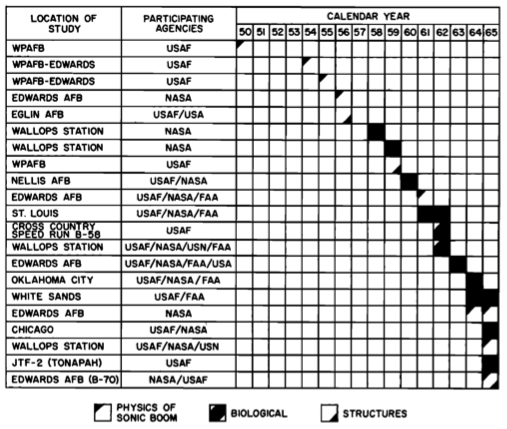
\includegraphics[width=\textwidth]{figs/research-status.png}
  \caption{History of operational sonic boom research from 1950-1965~\cite{nixon1965sonic}}
  \label{fig:research_status}
\end{figure}

One of the first experimental studies to include human response to sonic booms was conducted in Las Vegas in 1960 and outlined in a confidential report~\cite{maglieri1961ground}. This exploratory research sought to understand ``the possibility of doing enough damage as a result of the sonic boom to warrant its use as a tactical weapon against structures, equipment, and personnel.'' The experiment included recording near and far field pressures resulting from the sonic booms of two aircraft between Mach 1.05 and 1.16 for altitudes from about 50 to 890 feet. They researchers found that the wave shape from each plane was unique to the external geometry of the plane, see Figure~\ref{fig:shock_config}. Of the 214 window-glass breakage experiments performed, 51 damage points were obtained. The likelihood of damaging the glass increased as the pressure increased. 50 people were placed on the the minimum-altitude flightpath of the planes during the sonic booms. No harm was reported for pressures up to 120 lb/sq ft. Ear muffs were found to be useful in reducing the intensity of the noise, but were not found to be necessary. Some people reported a brief ringing in the ears following exposure, and it was expected that some small temporary hearing loss occurred. Follow-up experiments showed similar results, and again resulted no serious harm for pressures up to 144 lb/sq ft~\cite{nixon1968sonic}.

\begin{figure}[tb!]
  \centering
  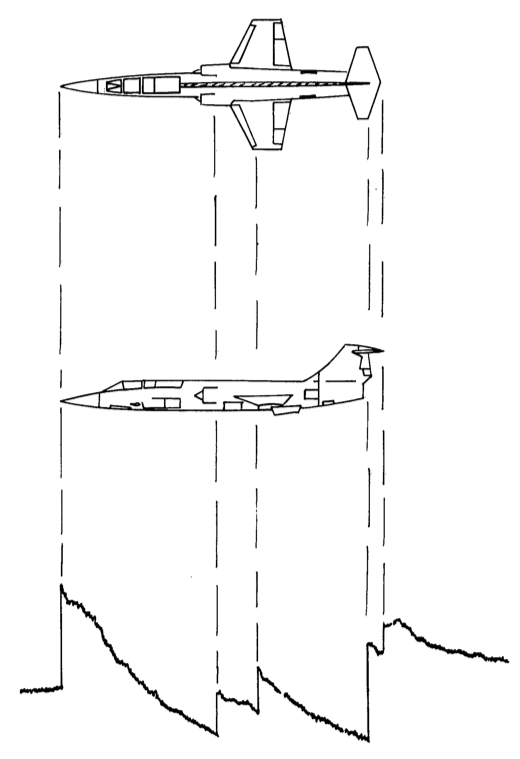
\includegraphics[width=0.9\textwidth]{figs/plane-shock-config.png}
  \caption{Top and side views of airplane with a typical time history of shock noise pressure~\cite{maglieri1961ground}}
  \label{fig:shock_config}
\end{figure}

These experiments showed that sonic booms were not physically damaging to humans, even when exposed at an extremely low altitude. Increasing interest in commercial supersonic transportation in the late 1960s led to further research into what intensity and frequency of sonic booms was acceptable by communities and society in general~\cite{nixon1965results, power1964sonic, nixon1966effects}. While no physical harm is caused by sonic booms, there is concern that sonic booms can interfere and annoy, causing startle and sleep disturbances. Unlike most loud noises, sonic booms are very sudden can even startle people used to experiencing them. There was additional concern that this startling effect could cause secondary problems due to resulting distraction. The community reaction repeated sonic booms is ``complex and highly variable and as such does not lend itself to firm predictive schemes nor inflexible exposure criteria~\cite{nixon1966effects}.'' Nixon continues, ``This response was not a function of overpressure alone but instead involved other elements of the stimulus exposure as well as a wide range of sociopsychological variables.'' While almost all residents report experiencing interferences with ordinary living activities, feelings of annoyance are generally fairly low, around 35\%.

Early investigations into the effects of sonic booms on humans found that, in general, there were fairly few negative side effects. As one community study from the mid-1960s claims ``[a]lthough millions of people were repeatedly exposed to sonic booms over a period of several months, no direct adverse physiological effects occurred and none was expected on the basis of existing knowledge.~\cite{nixon1966effects}'' These early studies provided important insight into the broad effects of sonic booms on humans, but did not include any laboratory studies of human perception. Several of these studies noted that overpressure alone was not sufficient to characterize the annoyance of the sonic booms, but none adequately define what metrics are necessary.

\section{Human Response to Noise}
\subsection{Human Auditory System}

\begin{figure}[tb!]
  \centering
  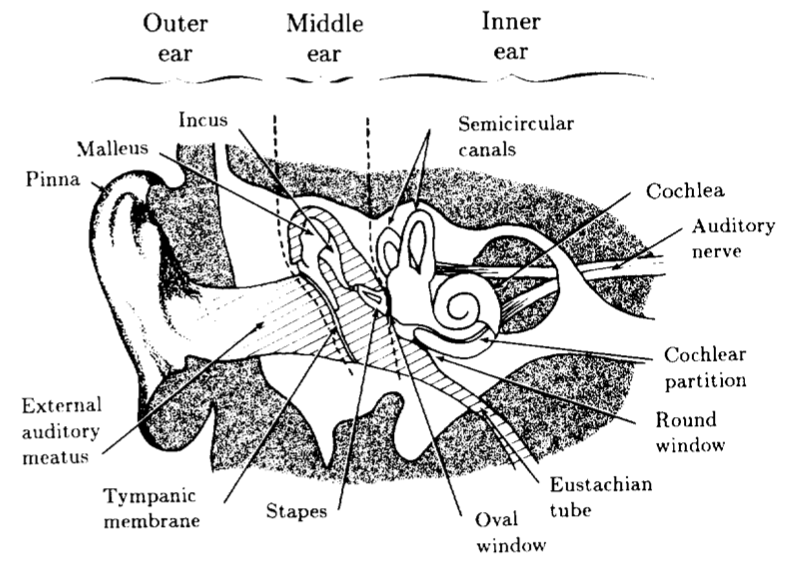
\includegraphics[width=\textwidth]{figs/ear-cross-section.png}
  \caption{Cross section of the human ear~\cite{powell1991human}}
  \label{fig:ear_cross}
\end{figure}

The human auditory system is capable of perceiving pressure fluctuations over a wide range of frequencies. There is not a one-to-one relationship between sound energy and any given noise effect, however, and it ``is necessary to thoroughly understand the physical characteristics of the sound and how each of those characteristics can affect human response.~\cite{powell1991human}'' Noise can have many adverse effects, including hearing loss, task performance degradation, speech intelligibility reduction, sleep interruption, and general feelings of annoyance. To understand how different characteristics of sound can cause these effects, it's first important to understand more about the perception of sound.

The auditory system consists of the outer, middle, and inner ears and the associated pathways to the brain, see Figure~\ref{fig:ear_cross}. Pressure fluctuations travel through the external auditory meatus and cause the the tympanic membrane to vibrate, which forms a mechanical linkage with the fluid in the inner ear. Vibratory motion in the fluid pass the traveling wave through the cochlear partition, ultimately exciting the hair cells on the basilar membrane. The excitation of the hair cells is transmitted to the brain via neural signals~\cite{powell1991human}.

Given the complicated process to transmit pressure waves to neural signals, it should not be surprising that the response of the auditory system is not easy to predict. Despite this complex system, some generalizations can be made~\cite{powell1991human}:
\begin{itemize}
\item Human auditory system is sensitive to a wide range of frequencies, from 20 Hz to 20 kHz
\item Nonuniform response over this range, with low sensitivity on both the lower and upper ranges
\item One sound can mask the perception of a lower intensity sound
\item High sound pressure levels can cause temporary and permanent shifts in hearing ability
\end{itemize}

\subsection{Noise Metrics}
There have been a variety of metrics used to predict the loudness, noisiness, and annoyance of sounds based off their characteristics. While the human auditory system is sensitive over a wide range of frequencies, the response is not flat over the entire range. Several techniques, the simplest of which are frequency weighting filters, have been created to predict the effects of noise based off their measurable characteristics.

\begin{figure}[tb!]
  \centering
  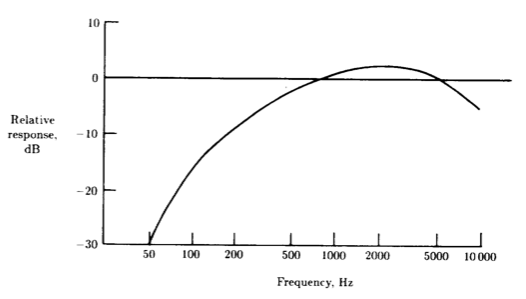
\includegraphics[width=\textwidth]{figs/sla.png}
  \caption{Relative response of the A-weighting filter~\cite{powell1991human}}
  \label{fig:sla}
\end{figure}

The loudness level of noise is commonly measured with the sound pressure level (SPL) modified by the A-weighting filter, resulting in the A-weighted sound level (SLA). SLA has been found to correlate very well noisiness and loudness of many sounds regardless of SPL~\cite{powell1991human}. The power at a certain frequency can be found by solving for the octave or 1/3 octave band SPL. To solve for a specific octave band frequency, the frequencies within that band can be added via
\begin{align}
L_A = 10 \log_{10} \left[ \sum_{i=1}^n 10^{L_A(i)/10} \right]
\end{align}
where $L_A(i)$ are the weighted SPL's of the frequency bands. Once the SPL is found at any specific frequency, the relative response from the A-weighting filter can be applied to approximate the perceived loudness.

While SLA is the simplest estimation of loudness, various loudness levels prediction schemes have been developed over the years~\cite{stevens1961procedure, zwicker1966comparison}. Stevens created a loudness levels ($LL_S$) scheme called Mark VI which accounts for some nonlinear effects in frequency characteristics. His loudness unit, sone, is defined as the loudness of a 1-kHz pure tone with a SPL of 40 dB~\cite{powell1991human}. The loudness in sones of each octave can be determined, and the total loudness can be found from summing
\begin{align}
S_t = S_m + F \left[ \sum_{i=1}^n S(i) - S_m \right]
\end{align}
where $S_m$ is the loudness of the loudest band, and F is an experimentally determined masking factor. The total loudness level in phons is calculated by
\begin{align}
L_L = 40 + 10 \log_2 S_t
\label{eq:ll}
\end{align}
Adjusting for nonlinear effects results in some improvement in experimental conditions over a simple SLA~\cite{stevens1961procedure}. The adjustment required by the A-weighting filter can be seen in Figure~\ref{fig:sla}. Zwicker developed another loudness level ($LL_Z$) scheme accounting for additional complexities in the human auditory system~\cite{zwicker1966comparison}. Initially developed for use to calculate loudness by hand for stationary sounds, computers then allowed the method to be used for nonstationary sounds~\cite{powell1991human}. After adjusting for ``critical bandwidth'' at low frequencies and different sensitivities to different types of sound fields, the final loudness level is calculated using Equation~\ref{eq:ll}~\cite{zwicker1966comparison}.

The perceived noise level (PNL) was initially developed to predict the reported annoying quality of jet aircraft sounds, and is the most commonly used metric to predict the noisiness level of sounds~\cite{kryter1959scaling}. PNL is calculated in a very similar manner to the loudness level, and the unit of perceived noisiness, noy, is defined as the noisiness of an octave band centered at 1 kHz with a SPL of 40 dB~\cite{powell1991human}. Similarly to the A-weighting filter, a D-weighting filter is commonly used to to adjust for the nonlinearities in the human auditory system. Comparing the A-weighting and D-weighting filters results in a large degree of similarity, see Figure~\ref{fig:d-weighting}. Similar to with loudness, $L_A$, the D-weighting is applied to the octave or 1/3 octave SPL's via
\begin{align}
L_D = 10 \log_{10} \left[ \sum_{i=1}^n 10^{L_D(i)/10} \right]
\end{align}
to produce a final D-weighted sound level (SLD). Extreme similarities in the loudness and noisiness had led researchers to propose that both are a result of the same auditory response~\cite{stevens1972perceived}. A perceived level (PL) was developed to calculate both loudness and nosiness using the same set of input data. After it was proposed that longer duration sounds were more annoying than shorter duration noises, the effective perceived noise level (EPNL) was established~\cite{noisestandards}. EPNL is used as a certification metric for new aircraft and engines.

\begin{figure}[tb!]
  \centering
  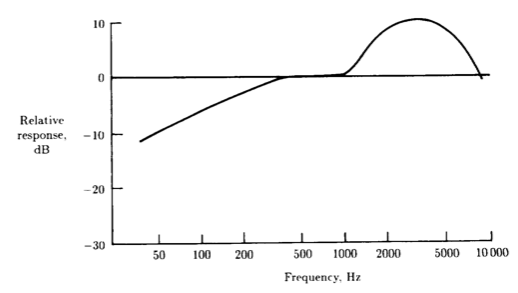
\includegraphics[width=\textwidth]{figs/d-weighting.png}
  \caption{Relative response of the D-weighting filter~\cite{powell1991human}}
  \label{fig:d-weighting}
\end{figure}

At least one serious experiment was completed to test the practical value of different noise metrics~\cite{ollerhead1971evaluation}. Up to 32 subjects took part in laboratory paired comparison tests to judge the perceived levels of 120 different aircraft flyover recordings. 18 different noise rating methods were selected as candidate metrics, with the primary objective of determining which methods were the most consistent. The experimenters tested different categories of aircraft sound, including turbojet (or fan) powered aircraft, propeller turbine aircraft, piston engined aircraft, and helicopters. Noise rating procedures were tested to determine how accurately and consistently subjects could measure perceived levels of sounds as compared to a standard reference of an octave band of noise centered at 1000 Hz~\cite{ollerhead1971evaluation}. They found that significant differences existed between different scales, and that the scales determined by Stevens, Zwicker, and Kyter performed the most consistently, though, with the exception of Zwicker's scheme, these scales overestimated the perceived level over the SPL range tested. The experimenters also found distinct differences in the applicability of different scales to the sounds in the four different aircraft categories~\cite{ollerhead1971evaluation}. Partial results of this experiment are reproduced in Figure~\ref{fig:noise-metrics}. Follow up studies to this experiment have found similar conclusions, with the $LL_Z$, $LL_S$ and PNL metrics performing approximately the same, and constantly outperforming other metrics~\cite{mccurdy1982annoyance, scharf1979comparison, powell1991human}. McCurdy and Clemans propeller and jet aircraft annoyance study used similar methodology and found that PNL, PL and $LL_S$ were somewhat superior to SLD and SLA~\cite{mccurdy1982annoyance}. Scharf and Hellman reanalyzed data from 23 studies of environmental noises and found that $LL_S$, PL, PNL, and $LL_Z$ generally better predicated loudness and acceptability than weighted metrics such as SLA, SLD, and SLE~\cite{scharf1979comparison}.

\begin{figure}[tb!]
  \centering
  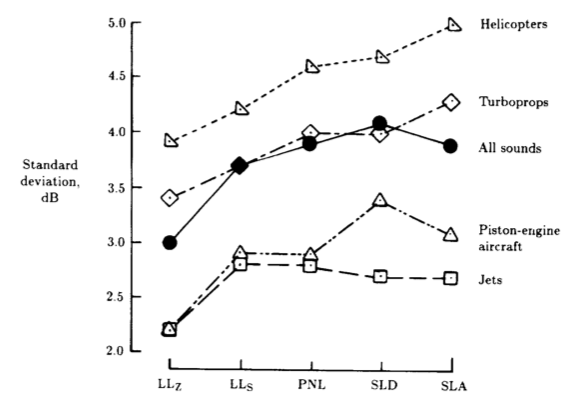
\includegraphics[width=\textwidth]{figs/noise-metrics.png}
  \caption{Prediction error for different noise metrics~\cite{ollerhead1971evaluation}}
  \label{fig:noise-metrics}
\end{figure}

\section{Sonic Booms}
Concern over the adverse effects of sonic booms has resulted in the prohibition of commercial supersonic flight over land within the United States~\cite{ollerhead1971evaluation}. There has been concern over the psychological and physiological response of humans and animals, as well as potential damage to structures and buildings. Additional concern into the effects of humans experiencing sonic booms, especially the startle response, has seen extra focus. In the early 1970s researchers were concerned with minimizing the possible undesirable effects on people of repeated sonic boom exposures~\cite{von1972human}. Various observations, overflight programs, and experimental field and laboratory studies were conducted in the United States and across other countries including France and the United Kingdom.

\begin{figure}[tb!]
  \centering
  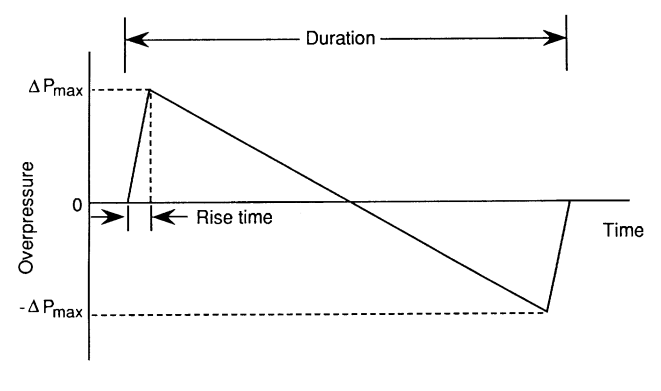
\includegraphics[width=\textwidth]{figs/n-wave.png}
  \caption{Parameters for N-wave Sonic Boom signatures~\cite{thackray1972sonic}}
  \label{fig:n-wave}
\end{figure}

\subsection{Laboratory Tests}

Laboratory tests found that loudness and annoyance of sonic booms are directly related to its energy spectral density function~\cite{johnson1969procedure}. Sonic booms are often modeled as N-waves. N-waves can be defined with just three parameters, peak overpressure, rise time, and duration, see Figure~\ref{fig:n-wave}. While peak overpressure is the most obvious contributor to loudness, it is not a sufficient factor. Rise time also plays an important role, and a decrease in rise time from 10 to 1 msec corresponds to a 13 dB increase in loudness~\cite{von1972human}. Relative annoyance and loudness are generally unaffected by N-wave signature durations, however, and durations ranging from 100 to 500 msec are generally considered the same. Except for very large rise times, of or above 10 msec, the annoyance and loudness are rated the same by human subjects. For rise times of 10 msec, however, the annoyance of subjects increases slightly more than the reported loudness. In general, decreases in rise time lead to larger loudness and annoyance, and N-wave duration has no apparent effect on either, see Figure~\ref{fig:n-wave-effects}.

\begin{figure}[tb!]
  \centering
  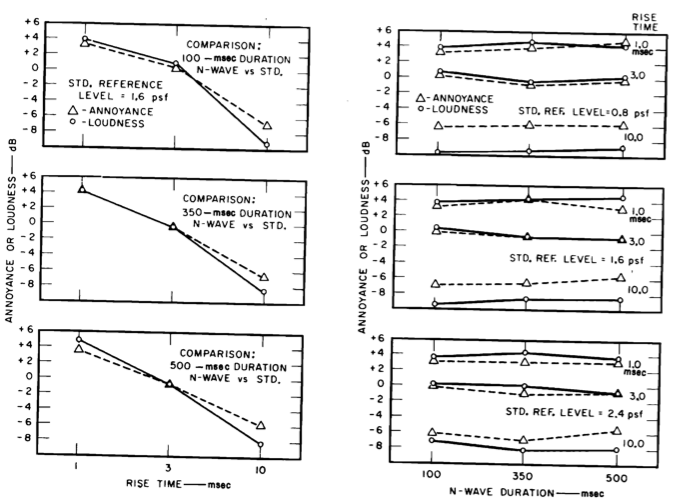
\includegraphics[width=\textwidth]{figs/n-wave-effects.png}
  \caption{Relative loudness and annoyance versus rise time of sonic booms from laboratory free-field judgments~\cite{von1972human}}
  \label{fig:n-wave-effects}
\end{figure}

Startle is one of the most considered physiological responses to sonic booms, and was investigated during a psychomotor tracking task~\cite{lukas1968preliminary}. Subjects were exposed to simulated sonic booms while controlling the manual task, and myographic responses (EMGs) were taken from the contrateral trapezius muscle. Subjects were divided into groups and given different amounts of sonic boom exposure before the task, in measure the effects of adaptation. While there were clear differences between the control and experimental groups, and subjects experienced some slight adaptation over the course of four sessions, see Figure~\ref{fig:startle}. Extrapolating the change in EMG response suggests that subjects would reach the levels in the control group after 7 to 9 sessions. Other authors have expressed interest in continuing this type of experiment, as it is unclear whether subjects will adapt to the control rates, or level off at a higher value~\cite{von1972human}.

Sonic booms have been found to have some effects on the quality of sleep in laboratory settings~\cite{lukas1968preliminary}. Indoor booms of varying magnitudes were generated inside of a laboratory where two subjects slept for a period of two weeks. Electroencephalograms (EEGs) were monitored continuously by the experimenters to both reveal sleep patterns and determine changes in these patterns as a result of sonic booms. Subjects were exposed to four different pressures of sonic booms at different stages of sleep. The loudest booms, at 1.6 and 2.1 psf, were found to cause significantly more wakings. Adaptation was seen for most phases of sleep, but even the quietest booms were found to wake sleepers during REM sleep. These same researchers later experimented with subjects of different age, from 7 to 72 years of age~\cite{sixsubjects}. They found large variations among subjects of the same age, and that subjects above the age of approximately 70 are much more likely than younger subjects to be awakened by younger subjects.

\begin{figure}[tb!]
  \centering
  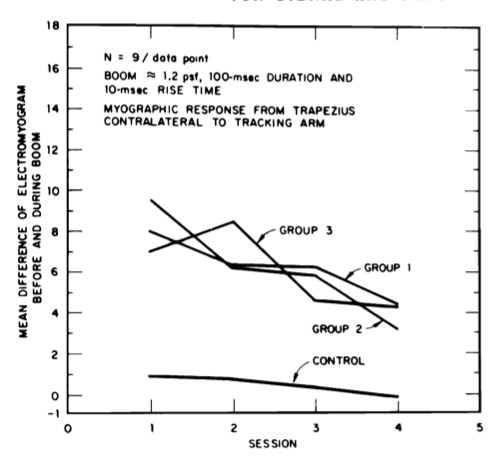
\includegraphics[width=\textwidth]{figs/startle.png}
  \caption{Mean normalized muscular startle response to simulated sonic boom as a function of test section~\cite{sixsubjects}}
  \label{fig:startle}
\end{figure}

\subsection{Indoor vs Outdoor Exposure}

\begin{figure}[tb!]
  \centering
  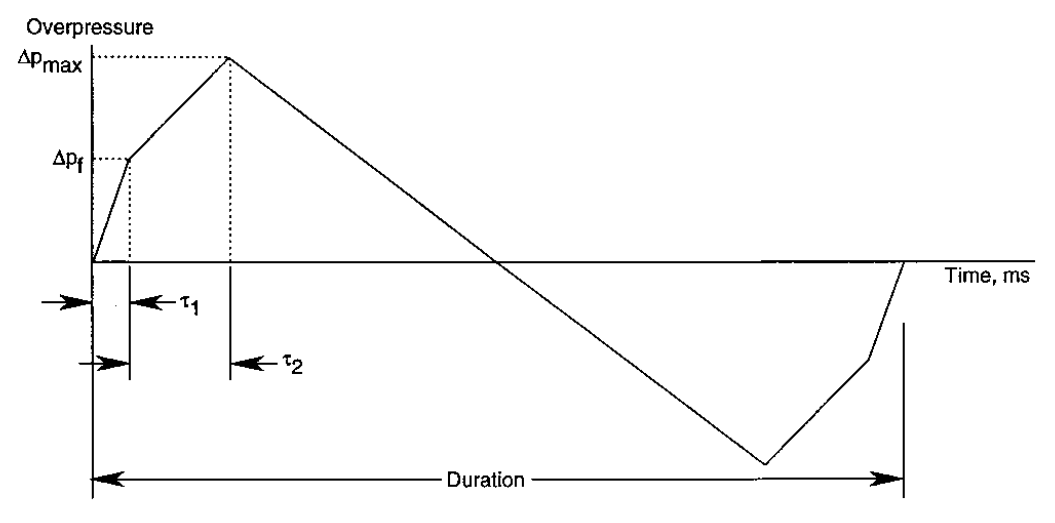
\includegraphics[width=\textwidth]{figs/fsm.png}
  \caption{Parameters for front-shock-minimized (FSM) sonic boom signatures. $\tau_1=$front-shock rise time, $\tau_2=$secondary rise time, $\Delta p_{max}=$peak overpressure, and $\Delta p_f=$front-shock overpressure~\cite{leatherwood2002summary}}
  \label{fig:fsm}
\end{figure}

\begin{figure}[tb!]
  \centering
  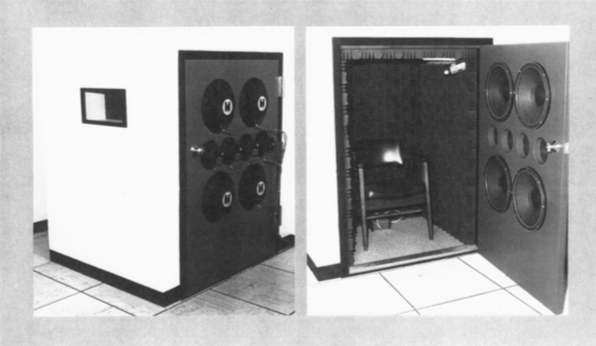
\includegraphics[width=\textwidth]{figs/langley-simulator.png}
  \caption{NASA Langley sonic boom simulator~\cite{leatherwood2002summary}}
  \label{fig:langley-simulator}
\end{figure}

\begin{figure}[tb!]
  \centering
  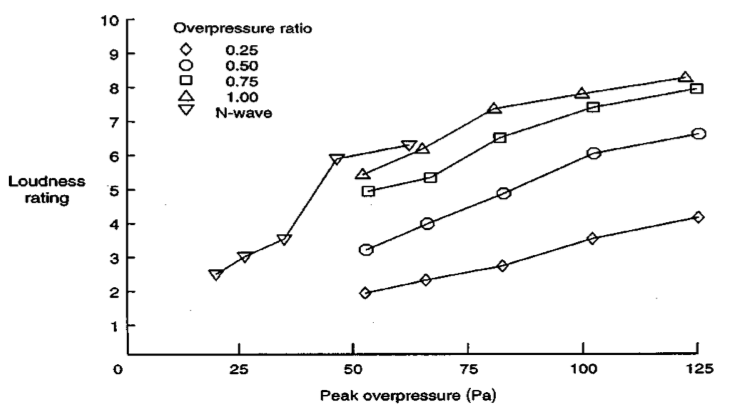
\includegraphics[width=\textwidth]{figs/fsm-comparison.png}
  \caption{Effect of peak overpressure level and overpressure ratio on subjective loudness for FSM signatures, $\tau_1=$1 ms~\cite{leatherwood2002summary}}
  \label{fig:fsm-comparison}
\end{figure}

Recent studies in the human perception of sonic booms have mainly focused on their perception indoors and the difference in their perception between in and outdoor exposure~\cite{leatherwood2002summary, sullivan2010human}. In addition to the N-waves discussed above, symmetrical front-shock-minimized (FSM) waveforms have also been tested. FSM waves compare well with the sonic boom waveforms experienced indoors. Leatherwood completed an experiment with sixty test subjects was conducted at the Langley Research Center sonic boom simulator to establish the effects of modifying the properties of FSM waveforms, see Figures~\ref{fig:fsm} and~\ref{fig:langley-simulator}~\cite{leatherwood1992laboratory}. These subjects rated the subjective loudness of 180 different waveforms on an 11-point numerical scale from ``not loud at all'' to ``extremely loud.'' Compared to the N-wave, all of the FSM waves were as quiet or quieter, with lower overpressure ratios resulting in lower loudness ratings~\cite{leatherwood2002summary}, see Figure~\ref{fig:fsm-comparison}.

\begin{figure}[tb!]
  \centering
  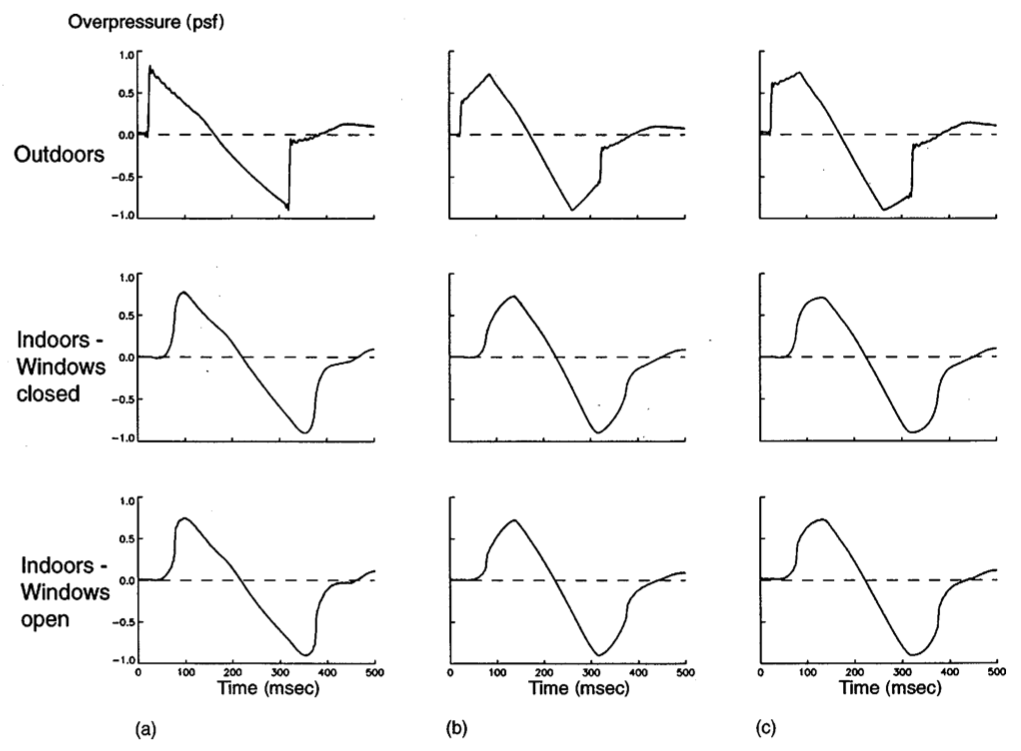
\includegraphics[width=\textwidth]{figs/indoor-outdoor.png}
  \caption{Boom signatures measured in simulator for three boom types and three simulated listening conditions. Boom types are (a) N waves, (b) FSM with overpressure ratio of 0.5, and (c) FSM with overpressure ratio of 0.75. Front-shock rise time for all boom types shown in 2 ms.~\cite{leatherwood2002summary}}
  \label{fig:indoor-outdoor}
\end{figure}

While the previous study showed that waveforms similar to what would be experienced indoors result in lower loudness than waveforms experienced outdoors, it was unclear how these effects would translate to reality. Much of the research into indoor sonic boom response is challenging ``because of room acoustics and wall attenuation effects, indoor waveforms generally lack distinctive rise time characteristics and lose significant high-frequency spectral energy. The result is an increase in relative emphasis of low-frequency spectral components of the indoor waveforms which could introduce annoyance components not present in outdoor waveforms.~\cite{leatherwood2002summary}'' Specifically, there is concern that wall, furniture, and the house in general can rattle, causing secondary noise which has the potential to be more annoying than the sonic boom itself.

Leatherwood followed up this experiment with another set of simulated indoor signatures derived from the application of house filters that approximated the noise reduction characteristics of a residential structure~\cite{leatherwood1993loudness}. Seventy two subjects were exposed to 135 simulated N-wave and FSM signatures. The results of this experiment were used to compare the differences between loudness and annoyance of sonic booms in outdoor and two indoor conditions. Two different house filters were used to simulate a typical residential structure with and without the windows closed. Example signatures for outdoors, indoors with windows closed, and indoors with windows open through three different overpressure ratios can be seen in Figure~\ref{fig:indoor-outdoor}. Figure~\ref{fig:simulated-comparisons} shows the relation between loudness and annoyance and perceived level for three simulated listening conditions. Fit lines for loudness and annoyance for the simulated outdoor waveforms were identical, implying that the outdoor waveforms did ``not contain annoyance components beyond those attributable to loudness.~\cite{leatherwood2002summary}'' Both indoor waveforms, especially the windows-closed waveform, show an increase in annoyance beyond the loudness values. This increase in annoyance is associated with an increased power in the low-frequency content. A PL increase in annoyance over loudness of 4.2 dB was seen for the windows-closed condition, and 1.6 dB was observed for the windows-open condition~\cite{leatherwood1993loudness}. The preferred subjective measurement is annoyance PL was recommended as the subjective sonic boom prediction metric based on these results, as loudness may not be sufficient.

\begin{figure}[tb!]
  \centering
  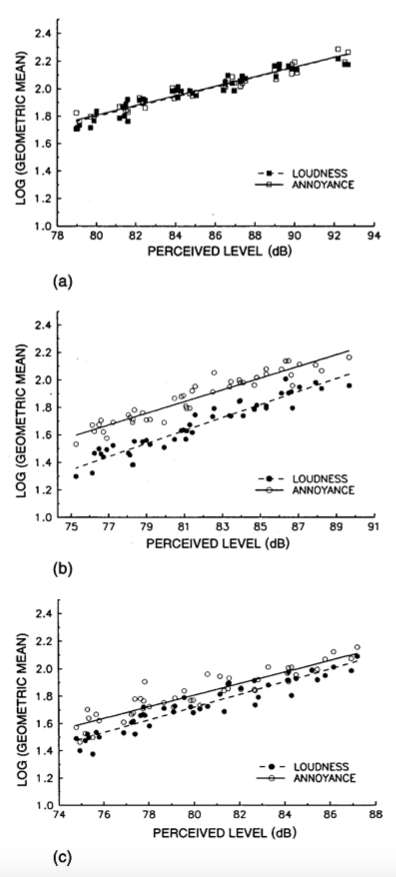
\includegraphics[width=0.6\textwidth]{figs/simulated-comparisons.png}
  \caption{Loudness and annoyance response comparisons for three simulated listening conditions: (a) outdoor condition; (b) indoor, windows-closed condition; and (c) indoor, windows-open condition~\cite{leatherwood2002summary}}
  \label{fig:simulated-comparisons}
\end{figure}

Recent research at Langley Research Center has included low-intensity sonic boom testing with subjects subjectively rating actual sonic booms inside and outside~\cite{sullivan2010human}. A total of 91 sonic booms were subjectively rated for annoyance by 77 subjects during an interval of four days. Before each sonic boom was scheduled, a reference test boom was played for the subjects to use as a basis measurement. For both the indoor and outdoor booms, the subjects sat in chairs in a V shape and could hear the reference sound from a speaker behind their head and the sonic booms could be recorded by a microphone placed to the speakers side, see Figure~\ref{fig:indoors-and-outdoors}. Of the 91 sonic booms used during the experiment, 20 were ultimately rejected due to excessive weather-related background noise, with 71 booms remaining with an acceptable signal-to-noise ratio~\cite{sullivan2010human}.

\begin{figure}[tb!]
  \centering
  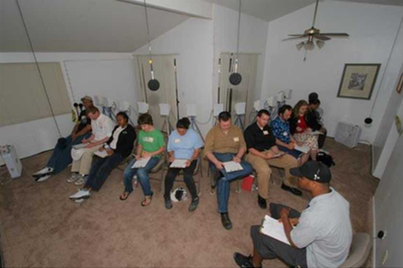
\includegraphics[width=0.8\textwidth]{figs/indoors.png}
  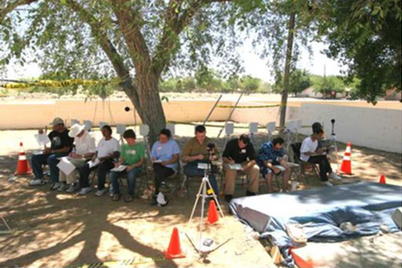
\includegraphics[width=0.8\textwidth]{figs/outdoors.png}
  \caption{Example experimental setup for twelve subjects to sit indoors and outdoors~\cite{sullivan2010human}}
  \label{fig:indoors-and-outdoors}
\end{figure}

Despite the initial expectation that the signal attenuation due to the house would cause decreased annoyance, the opposite result is found --- average annoyance indoors is larger than outdoors, see Figure~\ref{fig:indoor-outdoor-comparison}. For these results, only the 71 sonic booms with a sufficiently high signal-to-noise ratio were used. As the reference sound level was on average 2.2 dB higher outdoors than indoors, the difference was split, and 1.1 dB was added to the outdoor scores and reduced from the indoor scores. This effect can be seen between the raw data in Figure~\ref{fig:indoor-outdoor-comparison}(a) and the adjusted scores in Figure~\ref{fig:indoor-outdoor-comparison}(b). The corrected scores are plotted against PL and CSEL in Figures~\ref{fig:indoor-outdoor-comparison}(c) and (d). Despite some subjects reporting higher annoyance with indoor booms, average annoyance was the same indoors and outdoors. After each day of testing subjects were also asked to respond to a questionnaire which included the question, ``Today you heard sonic booms while you were inside the house and while you were outside. Thinking back, which were more annoying?'' 48 of the 77 subjects reported greater annoyance inside, which is extremely significant. These results are inconsistent with each other and with the results from simulated indoor and outdoor waveforms from Leatherwood. In their discussion, the researchers note that the house subjects were listening in was ``very loose and had highly pronounced rattling of doors and windows.'' It is not clear why subjects were more likely to report higher indoor annoyance on the questionnaire than the numerical annoyance scales. The researchers further suggest that ``the test methodology requires the test subjects to compare sonic booms with the reference sound. This may have had the effect that the subjects emphasized the acoustical attributes of the sonic booms and minimized other factors such as vibration and rattle.''

\begin{figure}[tb!]
  \centering
  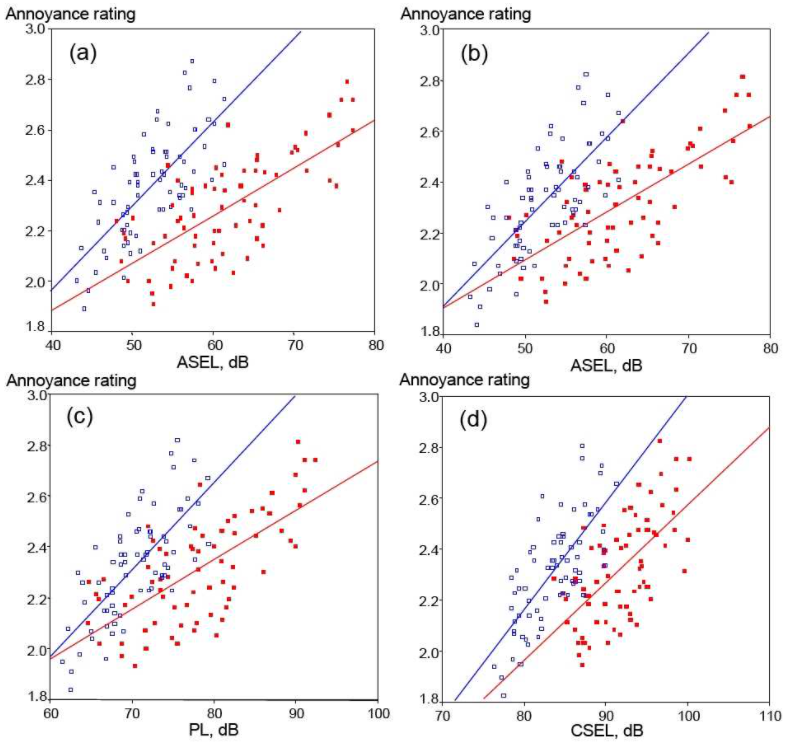
\includegraphics[width=\textwidth]{figs/indoor-outdoor-comparison.png}
  \caption{Annoyance response plotted against metric level, results for booms with SNR> 5 dB: (a) uncorrected annoyance ratings versus ASEL; (b) annoyance ratings corrected for reference sound level error versus ASEL; (c) annoyance ratings corrected for reference sound level error versus PL; (d) annoyance ratings corrected for reference sound level error versus CSEL. Blue: inside results, Red: outside results.
 ~\cite{sullivan2010human}}
  \label{fig:indoor-outdoor-comparison}
\end{figure}

\section{Summary and Conclusions}
Despite nearly 60 years of research into sonic booms and their physiological and psychological effects on humans remain largely unknown. While sonic booms were initially considered as a potential weapon to terrorize enemy infantry and destroy buildings, they did not fulfill this role. Sonic booms can shatter glass and cause lapses in concentration to those not adapted to their sounds. Sonic booms cause only slight, temporary hearing loss at distances as small as 50 feet, but are not very useful as a true weapon.

Extensive investigation into different metrics to quantify the spectral density functions associated with sonic booms. While some of the nonlinearities of the human auditory system have been captured, they are in no means complete. Zwicker's loudness level ($LL_Z$), however, has been found to be one of the most consistent schemes for minimizing discrepancies between subjects. N-waves and FSM signatures are often used to model sonic booms, but do not capture their non-symmetric effects. Despite this, they are useful as research tools, where shorter rise times have been shown to greatly increase loudness and annoyance.

The larger issue associated with sonic booms remains their limitation to not be used over populated areas. Individually, humans do not appreciate hearing sonic booms, and large populations have unpredictable and negative responses to them. Significant research has been completed to quantify the loudness and annoyance associated with booms, but the complications involved with modeling their expected physiological response are still lacking. While it appears that most people can adapt to hearing multiple sonic booms per day, response is highly variable. Additionally, there appears to be extreme sensitivity to sonic booms during REM sleep, especially among the elderly. There is inconclusive evidence that the annoyance associated with indoor sonic booms is higher than outdoor sonic booms, though some researchers cite incomplete metrics and difficulties associated with subject testing.

\bibliographystyle{ieeetr}
% \nocite{*}
\bibliography{bib}

\end{document}
